% -*- root: ../Neurocomputacion.tex -*-
\section{Redes neuronales sencillas para clasificación de patrones}
\subsection{Redes Hebb}
A lo largo de esta sección es frecuente encontrar tablas donde se muestran los resultados calculados por diferentes redes neuronales al estudiar ciertas entradas. Aunque se asume que la neurona de salida deberá devolver valores de tipo binario o bipolar según el valor de activación supere o no el umbral, en las tablas mostraremos por lo general el valor que ha recibido esa neurona de salida.

Esta decisión se debe a que facilita la comprensión del ejercicio y la comparación de este valor con el umbral es una tarea trivial que puede hacer el lector sobre la marcha.

\begin{problem}[1]
Apply the Hebb rule to the training patterns that define the XOR function.
\solution

Las \concept{redes neuronales Hebb} se caracterizan por la presencia de $n$ neuronas de entrada, una de salida y una neurona especial, conocida como ``bias'' que actúa como una neurona de entrada que siempre recibe el valor 1.

El entrenamiento de estas neuronas parte de la inicialización a 0 de todos los pesos de la red. Tras esto, y por cada vector de entrenamiento, ajustamos los pesos de la red según la ecuación:
\begin{equation}\label{eq:hebbRule}
w_i=w_i+x_iy
\end{equation}

siendo $y$ el valor esperado en la neurona de salida que estamos ajustando.

Si nuestra red tuviera varias neuronas de salida para cada una de ellas deberíamos aplicar el mismo procedimiento.

Ahora debemos ver como serán los datos de entrenamiento que definen la función XOR, que están recogidos en la siguiente tabla:
\begin{center}
\begin{tabular}{|c|c|c|}
\hline
\textbf{A} & \textbf{B} & \textbf{A XOR B}\footnote{Consideramos los valores de salida con una codificación bipolar ya que esta red no es capaz de aprender nada de aquellos patrones de entrenamiento con output nulo} \\
\hline
-1 & -1 & -1 \\
-1 & 1 & 1 \\
1 & -1 & 1 \\
1 & 1 & -1 \\
\hline
\end{tabular}
\end{center}

Es evidente ver que nuestra red tendrá un total de 4 neuronas siendo una de ellas la neurona de salida, por lo que nuestro vector de pesos inicializado será:
\[w = (0,0,0) \text{ siendo } w_0 \text{ el peso asociado al ``bias''}\]

Aplicando la ecuación \ref{eq:hebbRule} obtenemos el siguiente resultado:
\begin{center}
\begin{tabular}{|c|c|c|}
\hline
\textbf{Entrada} & \textbf{Vector de pesos antes} & \textbf{Vector de pesos despues} \\
$(x_1,x_2,y)$ & $(b,x_1,x_2)$ & $(b,x_1,x_2)$\\
\hline
(-1,-1,-1) & (0,0,0) & (-1,1,1)\\
(-1,1,1) & (-1,1,1) & (0,0,2)\\
(1,-1,1) & (0,0,2) & (1,1,1)\\
(1,1,-1) & (1,1,1) & (0,0,0)\\
\hline
\end{tabular}
\end{center}

No obtenemos un resultado válido puesto que la regla de Hebb sólo permite entrenar redes neuronales para problemas \concept{linealmente separables}, esto es, problemas en los que los puntos del espacio (en este caso un plano) que tienen salida positiva y los que tienen salida negativa pueden separarse linealmente.

En este caso concreto los puntos a estudiar ocupan los vértices de un cuadrado siendo los vértices opuestos\footnote{Al hablar de vértices opuestos de un cuadrado nos referimos a vértices diagonalmente opuestos.} los que dan el mismo valor de salida. Evidentemente, no hay ninguna linea que dibujar en el plano que me separe vértices de un cuadrado en dos bloques dejando los opuestos en el mismo lado de la línea.


\end{problem}

\begin{problem}[2]
There are 16 different logic functions (with two inputs and one output), of which 14
are linearly separable. Show that the Hebb rule can find the weights for all problems
for which weights exist, as long as bipolar representation is used and a bias is included.

\solution

Las dos funciones lógicas que no pueden ser representadas mediante una red Hebb son el XOR y su negado.

La demostración de este hecho se basa en la idea comentada al final del ejercicio anterior. Si tenemos los 4 vértices de un cuadrado y queremos dividirlos en dos grupos por medio de una linea recta esta linea deberá, lógicamente, atravesar el cuadrado. Una vez comenzamos a dibujar la recta, esta deberá atravesar un lado del cuadrado, separando los dos vértices contiguos en distintos grupos.

Es evidente comprobar que no hay forma de prolongar esta recta (no importa que pendiente tomemos) de forma que los dos vértices restantes queden cada uno al lado de su opuesto.

\end{problem}

\begin{problem}[3]
\ppart Consider character recognition using the Hebb rule. In Example 2.8, the "X" and
"0" used for training differed in all but four components. Show that the net will
respond correctly to an input vector formed from either the "X" or the "0" with
up to 20 components missing. (Whether it responds correctly, of course, is based on
your knowing which pattern you started with-you might prefer an "I don't know"
response. However, since the net input to the output unit is smaller the more components are missing, the "degree of certainty" of the response can also be judged.)

\ppart Mistakes involve one or more pixels switching from the value in the original
training pattern to the opposite value. Show that at approximately 10 mistakes, the
net will be seriously confused. (The exact number depends on whether any of the
mistakes occur in the pixels where the training patterns differ.)
Example 2.8 could be rephrased as an example of distinguishing the pattern X
from not-X (rather than specifically detecting X versus 0). Another pattern (for not X) that might be added to the net is:

\begin{center}
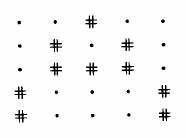
\includegraphics[width=0.3\textwidth]{img/pattern.png}
\end{center}

\ppart Find the new weights to store this pattern together with the two patterns used in
Example 2.8. (You can work from the weights in the example.) What does the bias
value tell you? How does the ability of the net to respond to noisy (missing or mis-
taken) data change as you add more patterns to the net? (You will probably need to
try more patterns of your own choosing in order to form a good conjecture to answer
this question.)

\solution
Atendiendo al ejemplo mencionado podemos observar que la idea consiste en escribir la cadena de símbolos que representa cada letra como un vector de 25 coordenadas, que será el input de nuestra red de Hebb.

Tras el breve proceso de entrenamiento (descrito en el ejemplo) se obtienen los pesos de las diferentes conexiones. Finalmente, podemos ver que la red considerará que ha leído una $X$ siempre que:
\[Σ = \begin{array}{ccccc}
2x_1& -2x_2 & -2x_3 & -2x_4 & +2x_5 +\\
-2x_6 & + 2x_7 &  & + 2x_9 &- 2x_{10} +\\
-2x_{11} & & +2x_{13} & & -2x_{15} + \\
-2x_{16} & +2x_{17} & & +2x_{19} & -2x_{20} + \\
+2x_{21} & -2x_{22} & -2x_{23} & -2x_{24} & +2x_{25} \\
\end{array} > 0\]

También nos indica el enunciado que, en caso de leer una $X$ perfecta, la suma anterior tiene valor $Σ=42$.

Es cómodo notar que, en esta ocasión, con la distribución de los pesos que acabamos de mostrar, las entradas que tendrán valor $1$ al leer la $X$ tienen pesos positivos y las que se activarán al leer el $O$ tienen valores negativos.
\spart
El primer apartado del problema nos pide comprobar que, aunque haya 20 casillas perdidas (es decir, 20 valores de entrada con valor 0), seguimos pudiendo detectar que se trataba de una $X$ (o de un $O$ respectivamente).

Basta con ver que cada dato que nos falte, salvo si es uno de los 4 valores asociados a un peso nulo, el valor de la neurona de salida decrece en dos unidades. Puesto que $Σ=42$, hasta 20 casillas sin información son toleradas, puesto que $Σ=42-2\cdot 20 > 0$\footnote{De hecho podrían faltar datos de incluso 24 casillas, si estas casillas son las adecuadas. No obstante, de forma general sólo podemos garantizar la correctitud de la red a la hora de clasificar el input si no faltan más de 20 datos}.
\spart
Por otro lado, es sencillo notar que un fallo en un valor, salvo en los casos en que el peso asociado a la neurona que lee ese valor es 0, implica una reducción en el valor de la neurona de salida de 4 unidades. Queda claro por tanto que $Σ=42-4\cdot 10>0$ por lo que hasta 10 errores son tolerados.

El mismo razonamiento partiendo de $Σ=-42$ que se ve aumentado con cada pérdida de información/error puede hacerse para el caso en que la entrada sea un $O$.

\spart
Vamos a completar ahora el entrenamiento de la red con el nuevo patrón que se nos proporciona. Recordando que el aprendizaje en las redes Hebb se lleva a cabo según la ecuación \ref{eq:hebbRule}, es sencillo comprobar que tras el último paso del entrenamiento tendremos:
\[Σ = -1 + \begin{array}{ccccc}
+3x_1& -1x_2 & -3x_3 & -1x_4 & +3x_5 +\\
-1x_6 & + 1x_7 & +x_8 & + 1x_9 &- 1x_{10} +\\
-1x_{11} & -x_{12} & +1x_{13} & -x_{14} & -1x_{15} + \\
-3x_{16} & +3x_{17} & +x_{18} & +3x_{19} & -3x_{20} + \\
+1x_{21} & -1x_{22} & -1x_{23} & -1x_{24} & +1x_{25} \\
\end{array}\]

Podemos comprobar que tras este entrenamiento el valor de la neurona de salida tras leer el patrón $X$ es $Σ=35$, con lo que se ha reducido la capacidad de detectar errores y fallos a la hora de clasificar el patrón $X$.

En general, a medida que añadamos patrones distintos de $X$ para el entrenamiento, habrá más distribuciones para las que el resultado Σ deba ser negativo. Por tanto cada vez menos ruido será necesario para hacer que la red clasifique mal un patrón $X$.
\end{problem}

\begin{problem}[4]
Create more letters, or different versions of X's and O's, for more training or testing
of the Hebb net.

\solution

Vamos a comprobar el resultado devuelto por la red al analizar los siguientes patrones:

\begin{center}
\begin{tabular}{|c|c|}
\hline
\textbf{Patrón} & \textbf{Clasificación} \\
\hline
 . \# \# \#  . & \\
\#  . \#  . \# & \\
\# \#  . \# \# & -35. No es una $X$\\
\#  . \#  . \# & \\
 . \# \# \#  . & \\
\hline
\#  .  .  .  . & \\
 . \#  .  .  . & \\
 .  . \#  .  . & 10. Se trata de una $X$ \\
 .  .  . \#  . & \\
 .  .  .  . \# & \\
\hline
\end{tabular}
\end{center}

\end{problem}

\begin{problem}[5]
\ppart Using the Hebb rule, find the weights required to perform the following classi-
fications: Vectors (1, 1, 1, 1) and ( - 1, 1, - 1, -1) are members of the class (and
therefore have target value 1); vectors (1, 1, 1, - 1) and (1, - 1, - 1, 1) are not
members of the class (and have target value -1).
\ppart Using each of the training x vectors as input, test the response of the net.
\solution

\spart
El proceso de entrenamiento de la red, que se realiza según la fórmula \ref{eq:hebbRule} queda ilustrado en la siguiente tabla:

\begin{center}
\begin{tabular}{|c|c|c|c|c|c|}
\hline
\textbf{Input} & \textbf{Target} & \textbf{Pesos antes} & \textbf{Bias antes} & \textbf{Pesos después} & \textbf{Bias después} \\
\hline
(1,1,1,1)    & 1  & (0,0,0,0) & 0 & (1,1,1,1) & 1\\
(-1,1,-1,-1) & 1  & (1,1,1,1) & 1 & (0,2,0,0) & 2\\
(1,1,1,-1)   & -1 & (0,2,0,0) & 2 & (-1,1,-1,1) & -1\\
(1,-1,-1,1)  & -1 & (-1,1,-1,1) & -1 & (-2,2,0,0) & 0\\
\hline
\end{tabular}
\end{center}

\spart
Vamos a comprobar que el entrenamiento ha funcionado, para ello debemos comprobar que el producto escalar del vector de pesos por el traspuesto del input nos da un valor positivo para aquellos input de la primera clase y negativo para los de la segunda.

\begin{center}
\begin{tabular}{|c|c|c|}
\hline
\textbf{Input} & \textbf{Target} & \textbf{Resultado} \\
\hline
(1,1,1,1)    & 1  & 0 \\
(-1,1,-1,-1) & 1  & 4 \\
(1,1,1,-1)   & -1 & 0 \\
(1,-1,-1,1)  & -1 & -4 \\
\hline
\end{tabular}
\end{center}

Podemos concluir que no se trata de un problema lineal puesto que el entrenamiento no da un resultado satisfactorio ni si quiera para los propios datos de entrenamiento.

\end{problem}

\begin{problem}[6]
\ppart The Hebb rule is sometimes used by converting the binary training patterns (inputs
and targets) to bipolar form to find the weight matrix. Apply this procedure to
find the weights to store the following classifications:
\begin{center}
s(1) = (1,0, 1), t(1) = 1\\
s(2) = (1, 1,0), t(2) = 0
\end{center}
\ppart Using the binary step function (with threshold 0) as the output unit's activation
function, test the response of your network on each of the binary training patterns.
\ppart Using the bipolar step function (with threshold 0) as the output unit's activation
function, convert the training patterns to bipolar form and test the network response again.
\ppart Test the response of your network on each of the following noisy versions of the
bipolar form of the training patterns:
\begin{center}
(0,-1,1) (0, 1, -1) (0, 0, 1) (0,0, -1) (0, 1,0) (0, -1,0)\\
(1, 0, 1) (1,0, -1) (1, -1,0) (1,0, 0) (1, 1,0) (1, 1, 1)
\end{center}
Which of the responses are correct, which are incorrect, and which are indefinite
(undetermined)?

\solution
\spart
Una vez más procedemos a entrenar una red de Hebb basándonos en datos de entrenamiento dados en forma bipolar. El resultado queda recogido en la siguiente tabla:
\begin{center}
\begin{tabular}{|c|c|c|c|c|c|}
\hline
\textbf{Input} & \textbf{Target} & \textbf{Pesos antes} & \textbf{Bias antes} & \textbf{Pesos después} & \textbf{Bias después} \\
\hline
(1,-1,1) & 1  & (0,0,0) & 0 & (1,-1,1) & 1\\
(1,1,-1) & -1 & (1,-1,1) & 1 & (0,-2,2) & 0\\
\hline
\end{tabular}
\end{center}

\spart
La red que acabamos de crear opera sobre los input dados (en binario) como muestra la siguiente tabla
\begin{center}
\begin{tabular}{|c|c|c|}
\hline
\textbf{Input} & \textbf{Target} & \textbf{Resultado} \\
\hline
(1,0,1) & 1  & 2\\
(1,1,0) & 0 & -2\\
\hline
\end{tabular}
\end{center}
Con lo que parece que el resultado obtenido es satisfactorio.

\spart
Operando sobre los datos de entrada en formato bipolar tenemos:
\begin{center}
\begin{tabular}{|c|c|c|}
\hline
\textbf{Input} & \textbf{Target} & \textbf{Resultado} \\
\hline
(1,-1,1) & 1 &  4\\
(1,1,-1) & 0 & -4\\
\hline
\end{tabular}
\end{center}
Con lo que parece que el resultado obtenido es satisfactorio.

\spart
Operando sobre los datos de entrada en formato bipolar tenemos:
\begin{center}
\begin{tabular}{|c|c|c|}
\hline
\textbf{Input} & \textbf{Target} & \textbf{Resultado} \\
\hline
(0,-1,1)   &  1 & 4 \\
(0, 1, -1) & -1 & -4 \\
(0, 0, 1)  &  1 & 2 \\
(0,0, -1)  & -1 & -2\\
(0, 1,0)   & -1 & -2\\
(0, -1,0)  &  1 & 2\\
(1, 0, 1)  &  1 & 2\\
(1,0, -1)  & -1 & -2\\
(1, -1,0)  &  1 & 2\\
(1,0, 0)   &  ? & 0 \\
(1, 1,0)   & -1 & -2\\
(1, 1, 1)  &  ? & 0\\
\hline
\end{tabular}
\end{center}

Los resultados esperados (columna Target) los he deducido buscando el vecino más próximo. Podemos comprobar que los resultados esperados coinciden exactamente con los obtenidos.

\end{problem}

\subsection{Perceptrón}

\begin{problem}[7]
Graph the changes in separating lines as they occur in Example 2.12.
\solution

Puesto que en esta ocasión el umbral es $\theta = 0$ sólo tendremos que dibujar una linea en cada iteración.

Por comodidad copiamos aquí la tabla que aparece en el ejemplo indicado, que recoge la evolución de los pesos de un perceptrón que está siendo entrenado para reconocer la función AND. El entrenamiento se realiza con entradas y salidas bipolares.


\begin{minipage}{0.4\textwidth}
\begin{center}
\begin{tabular}{|c|ccc|}
\hline
\textbf{Iteración} & & \textbf{Pesos} & \\
& $ω_1$ & $ω_2$ & $b$ \\
\hline
1 & 1 & 1 & 1\\
\hline
2 & 0 & 2 & 0\\
\hline
3 & 1 & 1 & -1\\
\hline
4 & 1 & 1 & -1\\
\hline
5 & 1 & 1 & -1\\
\hline
6 & 1 & 1 & -1\\
\hline
7 & 1 & 1 & -1\\
\hline
8 & 1 & 1 & -1 \\
\hline
\end{tabular}
\end{center}
\end{minipage}
\begin{minipage}{0.58\textwidth}
\begin{center}
\begin{tikzpicture}
\begin{axis}[
axis y line=center,
axis x line=middle,
axis equal,
grid=none,
xmax=5,xmin=-5,
ymin=-5,ymax=5,
xlabel=$ω_1$,ylabel=$ω_2$,
xtick=\empty,
ytick=\empty,
width=10cm,
anchor=center,
]
\addplot[no marks, color=red, very thick] {-x-1} ;
\addplot[no marks, color=blue, very thick] {0} ;
\addplot[no marks, color=green, very thick] {-x+1} ;
\addlegendentry{Iteración 1}
\addlegendentry{Iteración 2}
\addlegendentry{Iteración >3}
\end{axis}
\end{tikzpicture}
\end{center}
\end{minipage}

En los tres casos representados, el semiplano de aceptación es el que se encuentra por encima de la linea divisoria.
\end{problem}

\begin{problem}[8]
Explore the influence of the value of the learning rate on the speed of convergence
of perceptron learning:
\ppart Consider different values of α in Example 2.12; explain your results.
\ppart Modify the proof of the perceptron learning rule convergence theorem to include
an arbitrary learning rate a.
\solution

\spart

El ejemplo 2.12 se caracteriza por el empleo de un umbral $\theta = 0$. En este caso concreto, la modificación del valor α no tiene ningún efecto en la velocidad de convergencia del proceso de aprendizaje.

Para convencerse de ello basta con observar que lo único que nos importa es si el valor de salida de la red es mayor, menor o igual que 0. Puesto que empezamos con los pesos inicializados a 0, el efecto de cambiar α por un valor distinto simplemente modifica el valor neto obtenido en cada iteración pero no altera en absoluto la salida bipolar de la red.

La tabla representada en el ejemplo seguiría siendo la misma aunque los pesos aparecerían multiplicados por α, sea cual sea su valor (considerándolo siempre positivo)

\spart

Puesto que $ω(0)=0$ podemos tomar la demostración del libro y redefinir las funciones \textbf{w} y \textbf{x} empleadas en la demostración como: \textbf{w}$_2$ = α $\cdot$ \textbf{w}; \textbf{x}$_2$ = α $\cdot$ \textbf{x}.

El mínimo mencionado sigue existiendo (aunque ahora será un poco más pequeño, cosa que no nos afecta) y las desigualdades se mantienen.

Además, como seguimos considerando $\theta = 0$, la salida de la red neuronal en cada iteración no se ve alterada por la ponderación de los pesos (ni de los coeficientes de entrada). Así la desigualdad: \textbf{x}(k-1)$\cdot$\textbf{w}(k-1) $\leq 0$ empleada para reflejar la existencia de un error en la predicción de un valor del entrenamiento sigue manteniéndose con las nuevas  \textbf{x}$_2$ y \textbf{y}$_2$ puesto que el cambio de α no altera el signo de ningún valor.
\end{problem}

\begin{problem}[9]
 Show that the use of a bias is essential in Example 2.11. That is, show that it is
impossible to find weights W I and W2 for which the points (1,1), (1,0), (0,1), and (0,0)
are classified correctly. First, show that (0,0) will never be classified correctly, and
in fact, no learning will ever occur for that point. Then, neglecting (0,0), consider
whether (1,1), (1,0), and (0,1) can be classified correctly. That is, do weights WI and
W2 exist such that
\begin{center}
(1)$w_1$ + (1)$w_2$ > $\theta $ > 0,\\
(1)$w_1$ + (0)$w_2$ < $-\theta $ < 0,\\
(0)$w_1$ + (1)$w_2$ < $-\theta $ < 0
\end{center}
\solution

Sin tuviéramos $b=0$, tal y como está descrito el ejemplo 2.11, tendríamos siempre dos rectas de la forma:
\[y_1=ax+0.2 \text{ y } y_2 = bx - 0.2\]

El punto $(0,0)$ cumplirá siempre $y_1>0$ y $y_2<0$ por lo que no podrá ser clasificado correctamente.

Obviando este problema, vamos a ver qué ocurre con los otros puntos. Si existieran los valores $a$ y $b$ que dan lugar a las rectas descritas anteriormente, tendríamos:
\[\begin{array}{l}
1 > a+0.2 \\
1 > b-0.2 \\
a+0.2 > 0 \\
b-0.2 > 0 \\
0.2 > 1 \\
-0.2 > 1\\
\end{array}\]
donde las ecuaciones se obtienen al forzar que los puntos $(1,1), (1,0)$ y $(0,1)$ tengan los signos adecuados.

Finalmente, aunque las cuatro primeras ecuaciones dan lugar a la posibilidad de existir las rectas $y_1$ y $y_2$\footnote{Como es lógico puesto que si ignoramos el origen y uno de los puntos que se encuentran sobre los ejes es trivial ver que toda recta con pendiente menor que 1 (o mayor, según que punto del eje estemos ignorando) actúa como linea divisoria}, las dos últimas ecuaciones son inconsistentes.

\end{problem}

\begin{problem}[10]
Show that small initial weights still allow for any position of the initial decision line
for the perceptron.

\solution



\end{problem}

\begin{problem}[11]
 Repeat Example 2.11, and show that there is no change in the training process if
$\theta = 0$. Show that the separating line is
\[x_2=-\frac{2}{3}x_1+\frac{4}{3}\]
\solution

Es evidente que el cambio en el valor de $\theta$ indicado no cambia nada puesto que el valor calculado por la red, así como los pesos van a tener siempre valores enteros. Por tanto el único valor calculado por la red que de lugar a un output de 0 es el propio 0. Para el resto de valores calculados por la red, el output coincidirá con el signo del valor calculado.

Vamos a constuir la tabla correspondiente para ver cómo se comporta la red con $\theta = 0$

\begin{center}
\begin{tabular}{|c|c|c|c|c|c|c|}
\hline
\textbf{Input} & \textbf{Pesos antes} &  \textbf{Bias antes} & \textbf{Out} & \textbf{Target} & \textbf{Pesos después} & \textbf{Bias después} \\
\hline
( 1 , 1 , 1 ) & ( 0 , 0 ) &  0  &  0  &  1  & ( 1 , 1 ) &  1  \\
( 1 , 0 , 1 ) & ( 1 , 1 ) &  1  &  1  &  -1  & ( 0 , 1 ) &  0  \\
( 0 , 1 , 1 ) & ( 0 , 1 ) &  0  &  1  &  -1  & ( 0 , 0 ) &  -1  \\
( 0 , 0 , 1 ) & ( 0 , 0 ) &  -1  &  -1  &  -1  & ( 0 , 0 ) &  -1  \\
( 1 , 1 , 1 ) & ( 0 , 0 ) &  -1  &  -1  &  1  & ( 1 , 1 ) &  0  \\
( 1 , 0 , 1 ) & ( 1 , 1 ) &  0  &  1  &  -1  & ( 0 , 1 ) &  -1  \\
( 0 , 1 , 1 ) & ( 0 , 1 ) &  -1  &  0  &  -1  & ( 0 , 0 ) &  -2  \\
( 0 , 0 , 1 ) & ( 0 , 0 ) &  -2  &  -1  &  -1  & ( 0 , 0 ) &  -2  \\
( 1 , 1 , 1 ) & ( 0 , 0 ) &  -2  &  -1  &  1  & ( 1 , 1 ) &  -1  \\
( 1 , 0 , 1 ) & ( 1 , 1 ) &  -1  &  0  &  -1  & ( 0 , 1 ) &  -2  \\
( 0 , 1 , 1 ) & ( 0 , 1 ) &  -2  &  -1  &  -1  & ( 0 , 1 ) &  -2  \\
( 0 , 0 , 1 ) & ( 0 , 1 ) &  -2  &  -1  &  -1  & ( 0 , 1 ) &  -2  \\
( 1 , 1 , 1 ) & ( 0 , 1 ) &  -2  &  -1  &  1  & ( 1 , 2 ) &  -1  \\
( 1 , 0 , 1 ) & ( 1 , 2 ) &  -1  &  0  &  -1  & ( 0 , 2 ) &  -2  \\
( 0 , 1 , 1 ) & ( 0 , 2 ) &  -2  &  0  &  -1  & ( 0 , 1 ) &  -3  \\
( 0 , 0 , 1 ) & ( 0 , 1 ) &  -3  &  -1  &  -1  & ( 0 , 1 ) &  -3  \\
( 1 , 1 , 1 ) & ( 0 , 1 ) &  -3  &  -1  &  1  & ( 1 , 2 ) &  -2  \\
( 1 , 0 , 1 ) & ( 1 , 2 ) &  -2  &  -1  &  -1  & ( 1 , 2 ) &  -2  \\
( 0 , 1 , 1 ) & ( 1 , 2 ) &  -2  &  0  &  -1  & ( 1 , 1 ) &  -3  \\
( 0 , 0 , 1 ) & ( 1 , 1 ) &  -3  &  -1  &  -1  & ( 1 , 1 ) &  -3  \\
( 1 , 1 , 1 ) & ( 1 , 1 ) &  -3  &  -1  &  1  & ( 2 , 2 ) &  -2  \\
( 1 , 0 , 1 ) & ( 2 , 2 ) &  -2  &  0  &  -1  & ( 1 , 2 ) &  -3  \\
( 0 , 1 , 1 ) & ( 1 , 2 ) &  -3  &  -1  &  -1  & ( 1 , 2 ) &  -3  \\
( 0 , 0 , 1 ) & ( 1 , 2 ) &  -3  &  -1  &  -1  & ( 1 , 2 ) &  -3  \\
( 1 , 1 , 1 ) & ( 1 , 2 ) &  -3  &  0  &  1  & ( 2 , 3 ) &  -2  \\
( 1 , 0 , 1 ) & ( 2 , 3 ) &  -2  &  0  &  -1  & ( 1 , 3 ) &  -3  \\
( 0 , 1 , 1 ) & ( 1 , 3 ) &  -3  &  0  &  -1  & ( 1 , 2 ) &  -4  \\
( 0 , 0 , 1 ) & ( 1 , 2 ) &  -4  &  -1  &  -1  & ( 1 , 2 ) &  -4  \\
( 1 , 1 , 1 ) & ( 1 , 2 ) &  -4  &  -1  &  1  & ( 2 , 3 ) &  -3  \\
( 1 , 0 , 1 ) & ( 2 , 3 ) &  -3  &  -1  &  -1  & ( 2 , 3 ) &  -3  \\
( 0 , 1 , 1 ) & ( 2 , 3 ) &  -3  &  0  &  -1  & ( 2 , 2 ) &  -4  \\
( 0 , 0 , 1 ) & ( 2 , 2 ) &  -4  &  -1  &  -1  & ( 2 , 2 ) &  -4  \\
( 1 , 1 , 1 ) & ( 2 , 2 ) &  -4  &  0  &  1  & ( 3 , 3 ) &  -3  \\
( 1 , 0 , 1 ) & ( 3 , 3 ) &  -3  &  0  &  -1  & ( 2 , 3 ) &  -4  \\
( 0 , 1 , 1 ) & ( 2 , 3 ) &  -4  &  -1  &  -1  & ( 2 , 3 ) &  -4  \\
( 0 , 0 , 1 ) & ( 2 , 3 ) &  -4  &  -1  &  -1  & ( 2 , 3 ) &  -4  \\
( 1 , 1 , 1 ) & ( 2 , 3 ) &  -4  &  1  &  1  & ( 2 , 3 ) &  -4  \\
( 1 , 0 , 1 ) & ( 2 , 3 ) &  -4  &  -1  &  -1  & ( 2 , 3 ) &  -4  \\
( 0 , 1 , 1 ) & ( 2 , 3 ) &  -4  &  -1  &  -1  & ( 2 , 3 ) &  -4  \\
( 0 , 0 , 1 ) & ( 2 , 3 ) &  -4  &  -1  &  -1  & ( 2 , 3 ) &  -4  \\

\hline
\end{tabular}
\end{center}

Una vez hemos realizado todo el proceso de aprendizaje, es sencillo obtener la linea divisoria como:
\[x_1+3x_2-4 = 0 \implies x_2 = \frac{2}{3}x_1+\frac{4}{3}\]

\end{problem}

\begin{problem}[12]
 Consider carefully the difference in what can be solved using the following activation
functions:
\[f=\left\{ \begin{array}{ll}1 & \text{ if net } \geq \theta \\ 0 & \text{otherwise} \end{array}\right.\]
or
\[f=\left\{ \begin{array}{ll}1 & \text{ if net } \geq \theta \\ -1 & \text{otherwise} \end{array}\right.\]
or
\[f=\left\{ \begin{array}{ll}1 & \text{ if net } \geq \theta \\ 0 & \text{if} -\theta < \text{net} < \theta \\ -1 & \text{ if net } \leq -\theta\end{array}\right.\]
\solution

Considerando que estamos trabajando con un perceptrón (no lo especifica el enunciado pero estamos en la sección de problemas asociados al perceptrón) tendremos una función de activación (una vez hayamos entrenado la red) de la forma:
\[y = f(ω_0b + \sum_{i=1}^nω_ix_i) \]

Con las dos primeras funciones proporcionadas podemos resolver exactamente los mismos problemas. Lo que cambia es la codificación de la clasificación negativa por parte de la red. En estos casos podremos resolver todos aquellos problemas que sean linealmente separables.

En cuanto a la tercera función tendremos que los puntos estudiados se clasifican en tres tipos, según el valor de la neurona de salida respecto al umbral establecido. Esto nos permite resolver todos aquellos problemas que puedan separarse mediante dos rectas paralelas.

Por ejemplo, la función XOR, que no es separable, puede ser representada por un perceptrón que emplee una función como la tercera dada. Para ello basta con asociar la salida 1 y la salida -1 con la misma clasificación del patrón entrenado.

En el caso de la puerta lógica XOR que acabamos de mencionar tendríamos como solución:
\[y=f(-b + x_1+x_2) \text{ siendo } ω =0.5\]

\end{problem}

\begin{problem}[13]
 Even for $\theta= 0$, the perceptron learning rule prevents the correct classification of a point on the dividing line (which is better than assigning it arbitrarily to either side
of the line). If $\theta < α$ (the learning rate), does the exact value of $\theta$ matter? Does it matter if $\theta > α?$ Does it make a difference whether we start with all initial weights
equal to 0, as in Examples 2.11-2.13, or with other values (small random numbers,
for instance)?

\solution

El proceso de aprendizaje del perceptrón consiste en reajustar los pesos de la red \textbf{cuando se produzca un error en la predicción} según la fórmula:
\[ω_i = ω_i + αtx_i, \text{ siendo } t \text{ la salida esperada}\]

Esta regla sólo se aplica en los siguientes casos:
\[\begin{array}{lll}
\sum_{i=0}^nω_ix_i < -\theta & \text{ y } & t\geq 0 \\
\theta \geq \sum_{i=0}^nω_ix_i \geq - \theta & \text{ y } & \abs{t}> 0 \\
\sum_{i=0}^nω_ix_i > \theta & \text{ y } & t\leq 0
\end{array}\]

Podemos obviar aquellos casos en los que $t=0$ puesto que en esos casos no se produce ningún aprendizaje por lo que las preguntas planteadas por el enunciado carecen de sentido.

En el primer caso, tras corregir los pesos, ante la misma entrada, tendremos:
\[\sum_{i=0}^nω_ix_i + \sum_{i=0}^nαtx_i^2 \]
siendo
\[ \theta  k\leq  \sum_{i=0}^nαtx_i^2 \leq  αk\]
donde $k$ es el número de valores $x_i$ no nulos.

\textcolor{red}{No se cómo seguir a partir de aquí. Supongo que hay que jugar con estas desigualdades pero no se qué más hacer.}
\end{problem}

\begin{problem}[14]
 A variation of the perceptron learning rule allows active input units to increase their
weights and inactive units to decrease their weights in such manner that the total
weights are constant [see Block, 1962, p. 144, footnote 50]. Consider the effect this
would have on the binary representation of the AND function in Example 2.11.

\solution

No he sido capaz de encontrar en internet (sin pagar) la información de la referencia mencionada. No obstante, entiendo que se trata de modificar el algoritmo de aprendizaje del perceptrón de forma que las neuronas activas se potencien y las inactivas reduzcan su valor en caso de error.

Para implementarlo y generar la siguiente tabla, consideramos que el incremento en cada neurona activa será inversamente proporcional al número de neuronas activas. Del mismo modo el decremento en las entradas inactivas será inversamente proporcional al número de neuronas inactivas.

\begin{center}
\begin{tabular}{|c|c|c|c|c|c|c|}
\hline
\textbf{Input} & \textbf{Pesos antes} &  \textbf{Bias antes} & \textbf{Out} & \textbf{Target} & \textbf{Pesos después} & \textbf{Bias después} \\
\hline
( 1 , 1 , 1 ) & ( 0 , 0 ) &  0  &  0  &  1  & ( 0.75 , 0.75 ) &  0.75  \\
( 1 , 0 , 1 ) & ( 0.75 , 0.75 ) &  0.75  &  1  &  -1  & ( 1.75 , -0.75 ) &  1.75  \\
( 0 , 1 , 1 ) & ( 1.75 , -0.75 ) &  1.75  &  1  &  -1  & ( 0.25 , 0.25 ) &  2.75  \\
( 0 , 0 , 1 ) & ( 0.25 , 0.25 ) &  2.75  &  1  &  -1  & ( -0.75 , -0.75 ) &  4.25  \\
( 1 , 1 , 1 ) & ( -0.75 , -0.75 ) &  4.25  &  1  &  1  & ( -0.75 , -0.75 ) &  4.25  \\
( 1 , 0 , 1 ) & ( -0.75 , -0.75 ) &  4.25  &  1  &  -1  & ( 0.25 , -2.25 ) &  5.25  \\
( 0 , 1 , 1 ) & ( 0.25 , -2.25 ) &  5.25  &  1  &  -1  & ( -1.25 , -1.25 ) &  6.25  \\
( 0 , 0 , 1 ) & ( -1.25 , -1.25 ) &  6.25  &  1  &  -1  & ( -2.25 , -2.25 ) &  7.75  \\
( 1 , 1 , 1 ) & ( -2.25 , -2.25 ) &  7.75  &  1  &  1  & ( -2.25 , -2.25 ) &  7.75  \\
( 1 , 0 , 1 ) & ( -2.25 , -2.25 ) &  7.75  &  1  &  -1  & ( -1.25 , -3.75 ) &  8.75  \\
( 0 , 1 , 1 ) & ( -1.25 , -3.75 ) &  8.75  &  1  &  -1  & ( -2.75 , -2.75 ) &  9.75  \\
( 0 , 0 , 1 ) & ( -2.75 , -2.75 ) &  9.75  &  1  &  -1  & ( -3.75 , -3.75 ) &  11.25  \\
( 1 , 1 , 1 ) & ( -3.75 , -3.75 ) &  11.25  &  1  &  1  & ( -3.75 , -3.75 ) &  11.25  \\
( 1 , 0 , 1 ) & ( -3.75 , -3.75 ) &  11.25  &  1  &  -1  & ( -2.75 , -5.25 ) &  12.25  \\
( 0 , 1 , 1 ) & ( -2.75 , -5.25 ) &  12.25  &  1  &  -1  & ( -4.25 , -4.25 ) &  13.25  \\
( 0 , 0 , 1 ) & ( -4.25 , -4.25 ) &  13.25  &  1  &  -1  & ( -5.25 , -5.25 ) &  14.75  \\
( 1 , 1 , 1 ) & ( -5.25 , -5.25 ) &  14.75  &  1  &  1  & ( -5.25 , -5.25 ) &  14.75  \\
( 1 , 0 , 1 ) & ( -5.25 , -5.25 ) &  14.75  &  1  &  -1  & ( -4.25 , -6.75 ) &  15.75  \\
( 0 , 1 , 1 ) & ( -4.25 , -6.75 ) &  15.75  &  1  &  -1  & ( -5.75 , -5.75 ) &  16.75  \\
( 0 , 0 , 1 ) & ( -5.75 , -5.75 ) &  16.75  &  1  &  -1  & ( -6.75 , -6.75 ) &  18.25  \\
( 1 , 1 , 1 ) & ( -6.75 , -6.75 ) &  18.25  &  1  &  1  & ( -6.75 , -6.75 ) &  18.25  \\
( 1 , 0 , 1 ) & ( -6.75 , -6.75 ) &  18.25  &  1  &  -1  & ( -5.75 , -8.25 ) &  19.25  \\
( 0 , 1 , 1 ) & ( -5.75 , -8.25 ) &  19.25  &  1  &  -1  & ( -7.25 , -7.25 ) &  20.25  \\
( 0 , 0 , 1 ) & ( -7.25 , -7.25 ) &  20.25  &  1  &  -1  & ( -8.25 , -8.25 ) &  21.75  \\
( 1 , 1 , 1 ) & ( -8.25 , -8.25 ) &  21.75  &  1  &  1  & ( -8.25 , -8.25 ) &  21.75  \\
( 1 , 0 , 1 ) & ( -8.25 , -8.25 ) &  21.75  &  1  &  -1  & ( -7.25 , -9.75 ) &  22.75  \\
( 0 , 1 , 1 ) & ( -7.25 , -9.75 ) &  22.75  &  1  &  -1  & ( -8.75 , -8.75 ) &  23.75  \\
( 0 , 0 , 1 ) & ( -8.75 , -8.75 ) &  23.75  &  1  &  -1  & ( -9.75 , -9.75 ) &  25.25  \\
( 1 , 1 , 1 ) & ( -9.75 , -9.75 ) &  25.25  &  1  &  1  & ( -9.75 , -9.75 ) &  25.25  \\
( 1 , 0 , 1 ) & ( -9.75 , -9.75 ) &  25.25  &  1  &  -1  & ( -8.75 , -11.25 ) &  26.25  \\
( 0 , 1 , 1 ) & ( -8.75 , -11.25 ) &  26.25  &  1  &  -1  & ( -10.25 , -10.25 ) &  27.25  \\
( 0 , 0 , 1 ) & ( -10.25 , -10.25 ) &  27.25  &  1  &  -1  & ( -11.25 , -11.25 ) &  28.75  \\
( 1 , 1 , 1 ) & ( -11.25 , -11.25 ) &  28.75  &  1  &  1  & ( -11.25 , -11.25 ) &  28.75  \\
( 1 , 0 , 1 ) & ( -11.25 , -11.25 ) &  28.75  &  1  &  -1  & ( -10.25 , -12.75 ) &  29.75  \\
( 0 , 1 , 1 ) & ( -10.25 , -12.75 ) &  29.75  &  1  &  -1  & ( -11.75 , -11.75 ) &  30.75  \\
( 0 , 0 , 1 ) & ( -11.75 , -11.75 ) &  30.75  &  1  &  -1  & ( -12.75 , -12.75 ) &  32.25  \\
( 1 , 1 , 1 ) & ( -12.75 , -12.75 ) &  32.25  &  1  &  1  & ( -12.75 , -12.75 ) &  32.25  \\
( 1 , 0 , 1 ) & ( -12.75 , -12.75 ) &  32.25  &  1  &  -1  & ( -11.75 , -14.25 ) &  33.25  \\
( 0 , 1 , 1 ) & ( -11.75 , -14.25 ) &  33.25  &  1  &  -1  & ( -13.25 , -13.25 ) &  34.25  \\
( 0 , 0 , 1 ) & ( -13.25 , -13.25 ) &  34.25  &  1  &  -1  & ( -14.25 , -14.25 ) &  35.75  \\

\hline
\end{tabular}
\end{center}

\textcolor{red}{La tabla está mal pero es que no se cómo escribir el algoritmo decentemente, puesto que no se cual es el algoritmo en realidad}
\end{problem}

\begin{problem}[15]
 Using the perceptron learning rule, find the weights required to perform the following
classifications: Vectors (1, 1, 1, 1) and ( - 1, 1, - 1, - 1) are members of the class
(and therefore have target value 1); vectors (1 , 1, 1, -1) and (1, - 1, - 1, 1) are not
members of the class (and have target value -1) . Use a learning rate of 1 and starting
weights of O. Using each of the training x vectors as input, test the response of the
net.

\solution

\end{problem}

\begin{problem}[16]
Repeat Examples 2.18 and 2.19 using binary rather than bipolar vectors
\solution

\end{problem}

\begin{problem}[17]
Construct a multilayer net with two hidden units that will learn a given (binary) input pattern perfectly. The first hidden unit will have its weights equal to the input pattern and its threshold equal to the number of 1's in the input pattern. The second hidden unit is designed so that it will fire if its net input is less than or equal to the number of 1's in a given pattern. Combine the output from these two hidden units so that the output unit will fire if both hidden units are on. The point of this exercise is to observe that for p input training patterns, 2p hidden units will allow the net to learn every training pattern perfectly.

\solution

\end{problem}

\begin{problem}[18]
The XOR function can be represented as
\[x_1 \text{ XOR } x_2 \iff (x_1 \text{ OR } x_2 ) \text{ AND NOT }(x_1 \text{ AND } x_2)\]
Construct a MADALINE to implement this formulation of XOR, and compare it with
the MADALINE in Example 2.21.
\solution
\end{problem}

\begin{problem}[19]
Using the delta rule, find the weights required to perform the following classifications:
Vectors (1, 1, 1, 1) and (-1, 1, - 1, - 1) are members of the class (and therefore
have target value 1); vectors (1, 1, 1, - 1) and (1, - 1, - 1, 1) are not members of
the class (and have target value -1). Use a learning rate of .5 and starting weights
of O. Using each of the training x vectors as input, test the response of the net.
\solution
\end{problem}
